\paragraph{Построить заданную сеть и настроить в ней динамическую маршрутизацию.}
\begin{center}
    \begin{tabular}{|c|l|l|l|l|}
        \hline
        Device              & Interface & IP Address   & Mask          & Default Gateway \\
        \hline
        \multirow{3}{*}{R1} & Fa0/0     & 192.168.1.1  & 255.255.255.0 & N/A             \\
        \cline{2-5}
        ~                   & S0/0/0    & 12.0.0.1     & 255.0.0.0     & N/A             \\
        \cline{2-5}
        ~                   & S0/0/1    & 11.0.0.2     & 255.0.0.0     & N/A             \\
        \hline
        \multirow{4}{*}{R2} & Fa0/0     & 192.168.2.1  & 255.255.255.0 & N/A             \\
        \cline{2-5}
        ~                   & S0/0/0    & 12.0.0.2     & 255.0.0.0     & N/A             \\
        \cline{2-5}
        ~                   & S0/0/1    & 13.0.0.2     & 255.0.0.0     & N/A             \\
        \cline{2-5}
        ~                   & S0/1/0    & 10.0.0.2     & 255.0.0.0     & N/A             \\
        \hline
        \multirow{2}{*}{R3} & Fa0/0     & 192.168.3.1  & 255.255.255.0 & N/A             \\
        \cline{2-5}
        ~                   & S0/0/0    & 13.0.0.1     & 255.0.0.0     & N/A             \\
        \hline
        \multirow{3}{*}{R4} & Fa0/0     & 192.168.4.1  & 255.255.255.0 & N/A             \\
        \cline{2-5}
        ~                   & S0/0/0    & 10.0.0.1     & 255.0.0.0     & N/A             \\
        \cline{2-5}
        ~                   & S0/0/1    & 10.0.0.1     & 255.0.0.0     & N/A             \\
        \hline
        PC1                 & Fa0       & 192.168.1.10 & 255.255.255.0 & 192.168.1.1     \\
        \hline
        PC2                 & Fa0       & 192.168.2.10 & 255.255.255.0 & 192.168.2.1     \\
        \hline
        PC3                 & Fa0       & 192.168.3.10 & 255.255.255.0 & 192.168.3.1     \\
        \hline
        PC4.1               & Fa0       & 192.168.4.11 & 255.255.255.0 & 192.168.4.1     \\
        \hline
        PC4.2               & Fa0       & 192.168.4.12 & 255.255.255.0 & 192.168.4.1     \\
        \hline
        PC4.3               & Fa0       & 192.168.4.13 & 255.255.255.0 & 192.168.4.1     \\
        \hline
    \end{tabular}
\end{center}

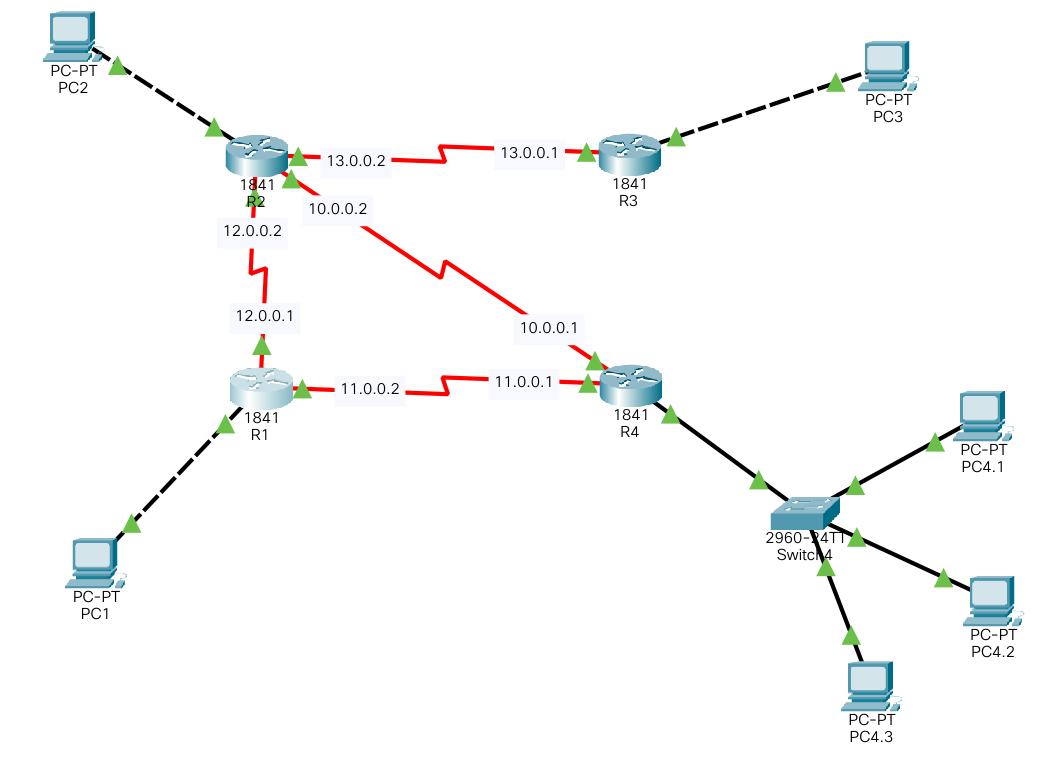
\includegraphics[width=0.9\textwidth]{resources/topology}
\lstinputlisting{resources/res}
\lstinputlisting{resources/ping}